\documentclass[border=4pt]{standalone}
\usepackage{amsmath,amssymb,amsfonts}
\usepackage{xcolor,colortbl,array,booktabs,multirow}
\usepackage{tikz}
\usepackage{pgfplots}
\pgfplotsset{compat=1.16}
\usetikzlibrary{arrows, automata, backgrounds, calendar, chains, decorations,
    matrix, mindmap, patterns, petri, positioning, shadows, shapes.geometric,
    trees, shapes, decorations.pathreplacing, calc, tikzmark, arrows.meta,
    intersections, fit, graphs, quotes, angles, decorations.markings}
\newcommand{\st}{\text{ s.t. }}
\newcommand{\x}{\mathbf{x}}
\renewcommand{\b}{\mathbf{b}}
\renewcommand{\c}{\mathbf{c}}
\newcommand{\A}{\mathbf{A}}
\newcommand{\y}{\mathbf{y}}
\newcommand{\z}{\mathbf{z}}
\newcommand{\R}{\mathbb{R}}
\newcommand{\RR}{\mathbb{R}}
\newcommand{\Z}{\mathbb{Z}}
\newcommand{\ZZ}{\mathbb{Z}}
\newcommand{\npcomplete}{NP-complete}
\providecommand{\true}{\text{TRUE}}
\providecommand{\false}{\text{FALSE}}
\tikzset{vertex/.style={circle,fill=black!25,minimum size=20pt,inner sep=0pt},
    edge/.style={draw,thick,-},weight/.style={font=\small},
    selected vertex/.style={vertex, fill=red!24},
    selected edge/.style={draw,line width=2pt,-,red!50},
    ignored edge/.style={draw,line width=2pt,-,black!20}}
\newcommand{\vect}{\vec}
\providecommand{\ds}{\displaystyle}
\providecommand{\longvect}{\overrightarrow}
\usepackage[normalem]{ulem}
\definecolor{ocre}{RGB}{243,102,25}
\providecommand{\leftB}{\left[}
\providecommand{\rightB}{\right]}
\tikzset{directed/.style={postaction={decorate,decoration={markings,mark=at position .65 with {\arrow{>}}}}},
    directed1/.style={postaction={decorate,decoration={markings,mark=at position .65 with {\arrow{>}}}}}}
\begin{document}
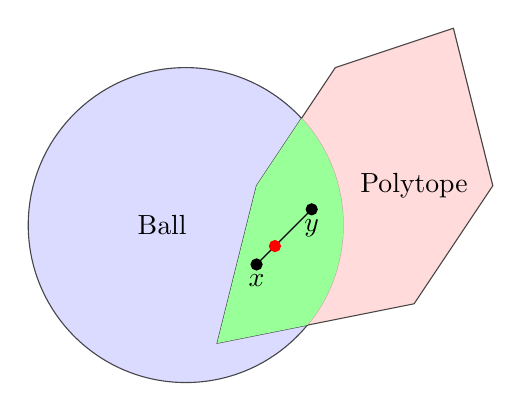
\begin{tikzpicture}

% Draw the circle (ball in 2D) slightly to the left
\filldraw[blue!20, opacity=0.7, draw = black] (0.1,1.5) circle (2cm);

% Draw the 6-vertex polytope slightly to the right
\filldraw[red!20, opacity=0.7, draw = black] (0.5,0) -- (3,0.5) -- (4,2) -- (3.5,4) -- (2,3.5) -- (1,2) -- cycle;

% Shade the intersection
\begin{scope}
  \clip (0.1,1.5) circle (2cm);
  \fill[green!40] (0.5,0) -- (3,0.5) -- (4,2) -- (3.5,4) -- (2,3.5) -- (1,2) -- cycle;
\end{scope}

% Label the circle and polytope
\node at (-0.2,1.5) {Ball};
\node at (3,2) {Polytope};

% Define the points
\coordinate (x) at (1,1);
\coordinate (y) at (1.7,1.7);
\coordinate (z) at (2/3*1 + 1/3*1.7, 2/3*1 + 1/3*1.7);

% Plot the line segment between x and y
\draw (x) -- (y);

% Mark the points with dots and labels
\filldraw [black] (x) circle (2pt) node[anchor=north] {$x$};
\filldraw [black] (y) circle (2pt) node[anchor=north] {$y$};
\filldraw [red] (z) circle (2pt) node[anchor=south east] {};%$z = \lambda x + (1-\lambda)y$};
\end{tikzpicture}
\end{document}
